\subsection{Objekterkennung}
\label{sec_objDet}
\subsubsection{Binärbild mit Template}
\todo{Kann man die graphen mit legends gut genug erkennen?}
Die Objekterkennung basiert auf einem ähnlichen Verfahren wie das vorgestellte CSurvey Projekt\cite{Albiez2015CSurveyA}.\\
Da ein Farberkennung aufgrund der Sichtbedingungen nicht in Frage kommt wird im ersten Schritt das RGB-Bild in ein Graustufenbild umgewandelt. Die erste Idee war es hier das Helligkeitsbild zu betrachten, da ein gesuchtes Objekt einen höheren Helligkeitswert besitzt, als der Meeresboden (siehe Abbildung \ref{brightCurve_real} und \ref{brightCurve_sim}).\\
Aus Erfahrungswerten früherer Projekte riet Christopher Gaudig mir, die Rotwerte der Bilder zu betrachten, da oftmals der Meeresboden und trübes Wasser geringe Rotwerte haben. In den Abbildungen \ref{redCurve_real} und \ref{redCurve_sim} ist dies zu beobachten. Die Kurven sehen denen der Helligkeitswerte sehr ähnlich, jedoch sind die Ausschläge des Objektes in den Rotwerten höher.\\
Im nächsten Schritt wird mithilfe eines Templates (Abbildung \ref{templImg}) ein Binärbild erzeugt. Das Template zeichnet sich durch drei Pixelangaben aus. Die \textit{Testpixel} (rot) geben einen Bereich an, der im aktuellen Schritt geprüft wird. Die \textit{Checkpixel} (blau) geben den Bereich rechts und links neben dem Testbereich an und bilden den Referenzwert. Die \textit{Borderpixel} (grün) geben einen Bereich zwischen Test- und Checkbereich an, der ignoriert wird. Jedes Pixel dient einmal als Mittelpunkt des Testbereichs, um zu entscheiden, ob das betrachte Pixel Teil des Objektes sein kann. Dies ist der Fall, wenn der Wert des Pixels [Gleichung \ref{templateValue}] einen Schwellwert (rote Linie) übersteigt.\\
%\begin{ownequation}[H]
%\begin{eqnarray}
%TP_i = \left\{i-\frac{\#TP}{2} \dots i \dots i+\frac{\#TP}{2}\right\}\\
%LC_i = \left\{i-\frac{\#TP}{2}-\#BP-\#CP \dots i-\frac{\#TP}{2}-\#BP\right\}\\
%RC_i = \left\{i-i+\frac{\#TP}{2}+\#BP \dots \frac{\#TP}{2}+\#BP+\#CP\right\}\\
%\end{eqnarray}
%\caption{Testbereich ($TP$) und Checkbereiche ($LC$ und $RC$) für ein Pixel mit Index $i$}
%\end{ownequation}
%Mit diesen Mengen lässt sich dann die Berechnung eines Templatewerts ($TV$) zu definieren.
%\begin{ownequation}[H]
%\begin{eqnarray}
%TV_i = \frac{\sum_{x \in TP_i} image(x))}{\#TP} - \left(\frac{\sum_{y_1 \in LC_i} image(y_1) + \sum_{y_2 \in RC_i} image(y_2)}{2 \cdot \#CP}\right)
%\end{eqnarray}
%\caption{Templatewertberechnung für ein Pixel $i$}
%\label{templateValue}
%\end{ownequation}

\begin{figure}[H]
\centering
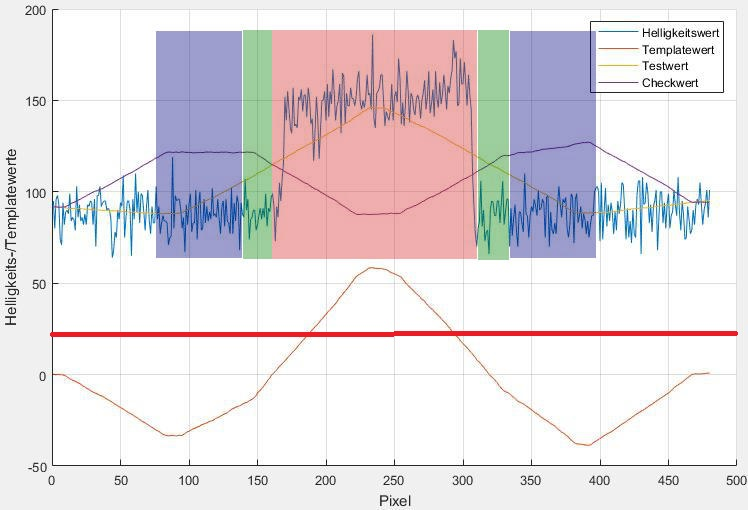
\includegraphics[scale=0.5]{imageProcessing/Prinzip/template.jpg}
\caption{Template zum Bestimmen des Binärbilds}
\label{templImg}
\end{figure}

\begin{ownequation}[H]
\begin{equation}
TV = \frac{sum(Testpixel)}{\#TP} - \frac{sum(Checkpixel)}{2 \cdot \#CP}
\end{equation}
\caption{Templatewertberechnung für ein Pixel}
\label{templateValue}
\end{ownequation}

\begin{figure}[H]
\begin{tabular}{cc}
\multicolumn{2}{c}{\subfloat[Originalbild]{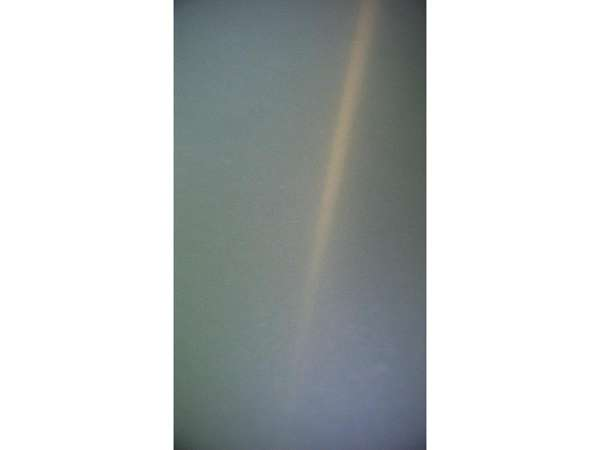
\includegraphics[height=0.33\textheight,width=\textwidth]{imageProcessing/realPipe/003orgImstart.jpg}}}\\
\subfloat[Helligkeitsverlauf einer Bildzeile im oberen Drittel des Bildes]{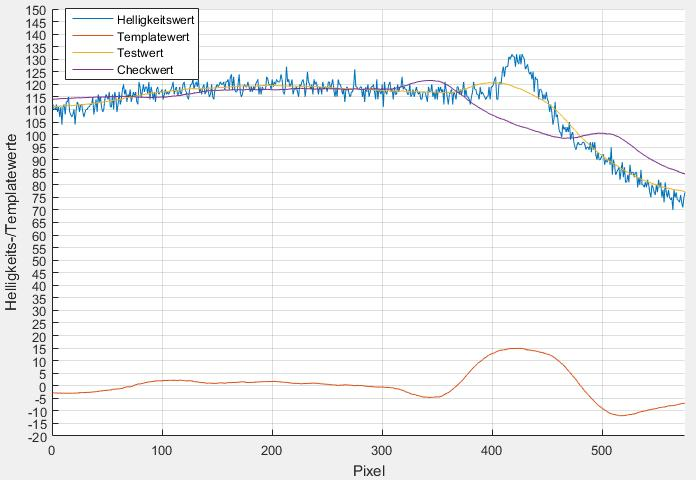
\includegraphics[height=0.33\textheight,width=0.5\textwidth]{imageProcessing/Prinzip/verkleinert/p3hellRealGut.jpg}\label{brightCurve_real}}&
\subfloat[Rotwertverlauf einer Bildzeile im oberen Drittel des Bildes]{\includegraphics[height=0.33\textheight,width=0.5\textwidth]{imageProcessing/Prinzip/verkleinert/p3rotRealGut.jpg}\label{redCurve_real}}
\end{tabular}
\caption{Helligkeit und Rotwert im echten Testbild}
\end{figure}

\begin{figure}[H]
\begin{tabular}{cc}
\multicolumn{2}{c}{\subfloat[Originalbild der Simulation]{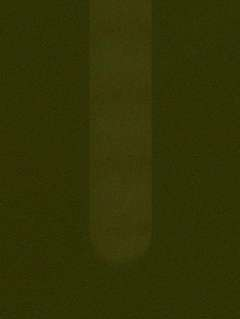
\includegraphics[height=0.33\textheight,width=0.4\textwidth]{imageProcessing/Prinzip/sim2,5Vis.jpg}}}\\
\subfloat[Helligkeitsverlauf einer Bildzeile im oberen Drittel des Bildes]{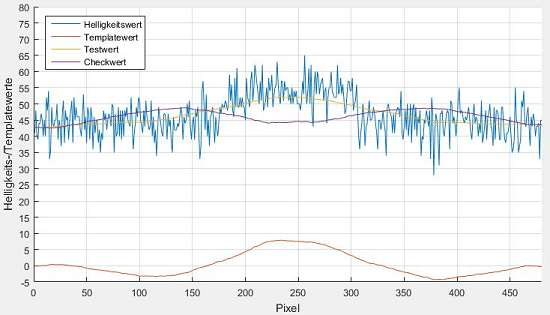
\includegraphics[height=0.33\textheight,width=0.5\textwidth]{imageProcessing/Prinzip/verkleinert/simHell2,5Vis.jpg}\label{brightCurve_sim}}&
\subfloat[Rotwertverlauf einer Bildzeile im oberen Drittel des Bildes]{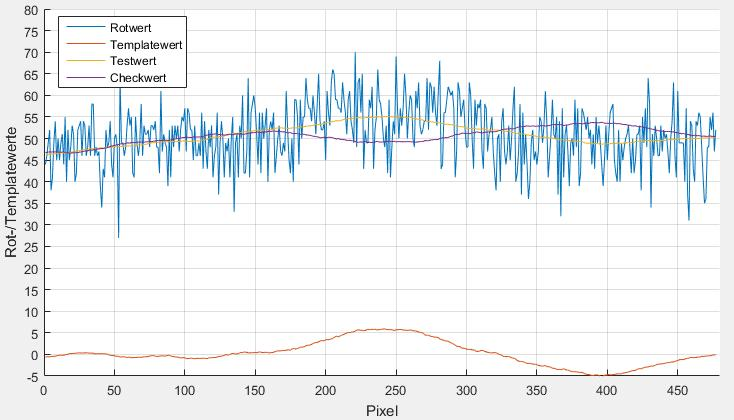
\includegraphics[height=0.33\textheight,width=0.5\textwidth]{imageProcessing/Prinzip/verkleinert/simRot2Vis.jpg}\label{redCurve_sim}}
\end{tabular}
\caption{Helligkeit und Rotwert im Simulationsbild}
\end{figure}

\subsubsection{Ransac auf Binärbild}
Im weiteren Verlauf wird auf dem  Binärbild gearbeitet. Nach dem Vorbild von Wang et al. \cite{wang2004lane} wird das Bild in drei Segmente unterteilt.\\
In jedem Segment wird dann mithilfe des \rans -Algorithmus ein Rechteck gesucht [Listing \ref{ransPseudo}]. Der Algorithmus sampled verschiedene Rechtecke im Segment. Dieses Rechteck wird durch einen Mittelpunkt, eine Orientierung, der Breite und der Höhe definiert. Die Höhe ergibt sich aus der Höhe des Segmentes und die Breite wird durch die erwartete Breite des Objektes festgelegt. Mittelpunkt und Orientierung werden in jedem Iterationsschritt zufällig gewählt.\\
Für jeden Punkt des Binärbilds wird dann geprüft, ob er im Rechteck liegt (ein Inlier ist). Gemäß des \rans wird das Rechteck mit den meisten Inliern gewählt.\\
\begin{lstlisting}[language=Matlab,caption=Eingesetzter Ransac als Pseudocode,label=ransPseudo]
function ransac(segment,height,width,minInlier,iterNum)
	maxInlier = 0;
	orientations = -pi/4:0.05:pi/4;
	bestCenter = None;
	bestOrientation = None;
	for i = 1:iterNum
		boxCenter = selectRandomPoint(segment);
		boxOrientation = selectRandomValue(orientations);
		inliers = findPointsInBox(segment, box=[boxCenter,boxOrientation,height,width]);
		
		if(len(inliers) > minInlier && len(inliers) > maxInlier)
			maxInlier = len(inliers)
			bestCenter = boxCenter;
			bestOrientation = boxOrientation;
		end
	end
end
\end{lstlisting}

Somit gibt es für jedes Bild bis zu drei Objektposen. Durch das unterteilen in Segmente lässt sich zum Einen bestimmen, in wie vielen Segmenten ein Objekt erkannt wurde (entspricht der \textit{Länge} des Objektes im Bild). Des weiteren kann ein gebogener Verlauf oder ein abgeknicktes Objekt im Bild sinnvoll erkannt werden.\\
In den ersten Tests dieses Verfahrens ist ersichtlich geworden, dass es einen \todo{richtige wortwahl?}Tradeoff zwischen Geschwindigkeit und Erkennungsgüte gab. Die Erkennung wurde besser, je mehr maximale Iterationen dem \rans erlaubt wurden. Da der \rans jedoch auf jedes der drei Segmente separat angewendet wird, wird bei steigender Iterationsanzahl die Geschwindigkeit deutlich reduziert. Für eine zuverlässige Erkennung waren zu viele Iterationen nötig, sodass das Verfahren nicht einsetzbar wäre.\\
Als Lösung für dieses Probleme habe ich die möglichen erzeugten Rechtecke für den \rans begrenzt. Da das Template nur in horizontaler Richtung auf das Bild angewendet wird, sind horizontal liegende Objekte im Binärbild nicht sichtbar. Aufgrund dieser Tatsache lassen sich die Orientierungen auf einen Bereich begrenzen, anstatt diese komplett zufällig zu wählen. Durch diese Maßnahme wurden die benötigten Iterationen für ein zuverlässiges Ergebnis drastisch reduziert. Jedoch steigt auch die Gefahr Orientierungen nicht mehr richtig zu erkennen, wie in Abbildung \ref{detecFail} gezeigt.\\
\begin{figure}[H]
\centering
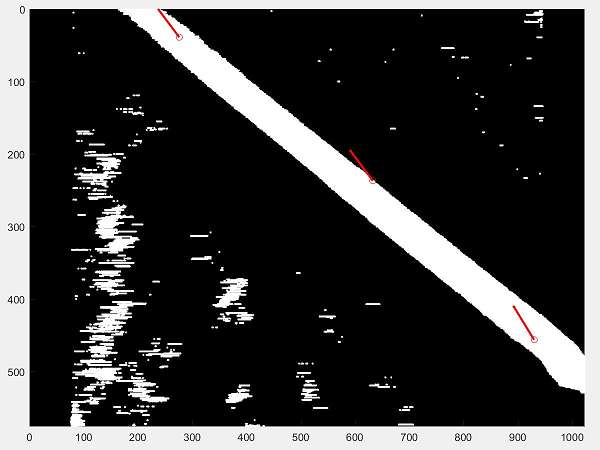
\includegraphics[scale=0.5]{imageProcessing/realPipe/004detectedImage.jpg}
\caption{Falsche Erkennung aufgrund der Beschränkung der Ausrichtungen für den \rans}
\label{detecFail}
\end{figure}
Der zweite Faktor, der die Geschwindigkeit der Objekterkennung verringerte war die Menge der Punkte im Binärbild. So musste für jede Iteration des \rans für jeden Punkt geprüft werden, ob der Punkt im Rechteck liegt. In den Testbildern der Simulation lag die Anzahl der Punkte teilweise bei weit über $10000$, was in Kombination mit $200$ Iterationen zu einer inakzeptablen Laufzeit von ca. 5 Sekunden pro Bild.\\
Zum Lösen dieses Problems wurden vorm Einsatz des \rans die Punktanzahl verringert, indem nur jedes dritte Pixel betrachtet wird und diese den Wert aller seiner Nachbarpixel erhält. \todo{Grafik?} Somit konnte die Punktanzahl zuverlässig auf unter $2000$ verringert werden, was zu einer deutlichen Beschleunigung (ca. 1 Sekunde pro Bild) ohne nennenswerte Verschlechterung der Ergebnisse führte.
%\subsubsection*{Gewicht der erkannten Punkte}
%\label{sec_weights}
%\begin{itemize}
%\item \textbf{numParts:} Länge des Objektes im Bild. Die erkannten Punkte werden nach Parallelität ihrer Ausrichtung und Nähe zueinander untersucht. Somit wird untersucht in wievielen Segmenten das Objekt fortgeführt wird.
%\item \textbf{area:} Um den Punkt wird ein Rechteck gelegt, dass der Breite des Objektes und der Höhe des Segmentes entspricht. \textbf{area} gibt einen relativen Wert an, wie ausgefüllt dieses Rechteck ist.
%\item \textbf{peakheight:} Es wird der Mittelwert aller der Helligkeit innerhalb des Rechtecks berechnet und mit dem allgemeinen Helligkeitswert des Bildes verglichen. \textbf{peakheight} dieses Verhältnis relativ an.
%\item \textbf{fitsBorder:} Gibt als boolean an, ob das erkannte Objekt der berechneten Objektbreite passt.
%\item \textbf{relativeCount:} Gibt das Verhältnis von Punkten im Binärbild, die zum Objekt passen und der Gesamtzahl der Punkte an.
%\end{itemize}